\documentclass[11pt,a4paper]{article}
\usepackage[T1]{fontenc}\usepackage[utf8]{inputenc}\usepackage[scaled=0.95]{helvet}\renewcommand{\familydefault}{\sfdefault}
\usepackage[a4paper,margin=2.2cm]{geometry}\usepackage{graphicx,booktabs,amsmath,caption}\usepackage[hidelinks]{hyperref}
\captionsetup{font=small,labelfont=bf}\setlength{\parindent}{0pt}\setlength{\parskip}{0.6em}
\begin{document}
{\LARGE\textbf{How many cars queue behind a cyclist in a shared winter lane on rue de Terrebonne?}}\\[4pt]
{\small Terrebonne-open-sources, 2026-11-08. Author: a resident of Côte-des-Neiges--Notre-Dame-de-Grâce (see the repository\textquoteright{}s « About the author »). Companion to the notes on street width, winter counts and parking. Data: the borough\textquoteright{}s loop counter (request 2026-300) and Miovision count (request 2026-634), the City géobase (CC-BY 4.0). Code, tables and figures: \url{https://github.com/OpenMobilityData/Terrebonne-open-sources/tree/main/2026-shared-lane-queue}.}

\section*{Abstract}
In the winter layout put to the borough council on November 2, 2026 (file 1266880005), cyclists riding in the direction of motor traffic would share the traffic lane with cars; in the layout drawn by the borough\textquoteright{}s consultant in 2023, that lane is 3.5\,m wide between two rows of parked cars. A driver may pass a cyclist only with the clearance of art.~341 of the Highway Safety Code, which such a lane does not leave, so a driver who catches up stays behind. This note estimates how many cars build up behind one cyclist at the winter morning peak. The borough\textquoteright{}s loop counter at Kensington recorded, on the 87 winter weekdays of 2025--26, a mean of 120 motor vehicles in the busiest morning hour (160 on a busy day, 90th percentile) and 3.6 eastbound bicycles; the Miovision count at Grand on January 29, 2025 gives 128 eastbound cars an hour between 07:00 and 09:00, of which 18\,\% turned off. Cars catch up with a slower cyclist at a rate set by the flow and the two speeds, and leave the queue when they turn off at a cross street. With a cyclist at 15\,km/h and cars at 25\,km/h (stops included) and 7\,\% of queued cars turning off at each of the 17 cross streets between Cavendish and Girouard, a cyclist is caught by 3.2 cars per kilometre and has 2.2 cars behind after 1\,km and 2.8 after the 1.5\,km to Girouard (simulation: median 3, 10th--90th percentiles 1--5). Across the range of assumptions the queue after 1\,km runs from 0.6 to 6.1 cars, and to 8.4 over the whole stretch on a busy morning with a slow cyclist. Seen from the drivers\textquoteright{} side, about 12 of the 120 cars of the peak hour (10\,\%) would follow a cyclist, each losing at most 1.6\,min per kilometre. The speeds are assumptions, not measurements, and the turn-off share comes from one intersection; the result is a range, not a measurement.

\section*{Lay summary}
In the borough\textquoteright{}s winter layout, cyclists going the same way as the cars would ride in a traffic lane too narrow for a car to pass them with the one metre the law requires, so drivers who catch up stay behind. Using the borough\textquoteright{}s counter (about 120 cars an hour at the winter morning rush) and assumed speeds of 15 km/h for the cyclist and 25 km/h for cars, a cyclist typically has two or three cars behind by Girouard: about one on a quiet morning, about eight on a busy one with a slow cyclist on snow. About 12 of the 120 peak-hour cars would follow a cyclist, each losing at most about a minute and a half per kilometre.

\tableofcontents

\section{Question}
The borough\textquoteright{}s offer to City council of November 2, 2026 (file 1266880005, p.~3) describes the winter measure: « retirer, durant la période hivernale, la bande cyclable située dans le même sens que la circulation véhiculaire afin de permettre son utilisation comme bande de stationnement. Les cyclistes circulant dans le même sens que la circulation seraient alors appelés à partager la voie de circulation avec les véhicules motorisés. » The only drawing of such a layout on the public record is the consultant\textquoteright{}s Aménagement~A (EXP, 2023, Figure~6-6, p.~72): a 3.5\,m lane between two 2.4\,m parking lanes. The street-width note in this repository measures the roadway at 11.0\,m curb to curb.

The question here is not whether a car fits beside a cyclist, which the street-width note addresses, but what happens when it does not: how many cars build up behind one cyclist, at the hour when most of them ride.

\section{The rules that apply}
Highway Safety Code (LégisQuébec, text current to October 15, 2026):
\begin{itemize}
\item art.~341: a driver may pass a cyclist in the same lane only with a reasonable distance, at least 1\,m where the limit is 50\,km/h or less (Terrebonne is posted at 30\,km/h); otherwise the driver stays behind.
\item art.~487: the cyclist rides as near the right edge as possible, taking into account the state of the roadway and the risk of dooring.
\item On a street designated as a vélorue by a municipality (arts.~496.1--496.8), a cyclist may ride on the full width of the lane (art.~496.8); art.~341 applies, but a driver is exempt from the distance where there is enough room to pass without danger (art.~496.3).
\end{itemize}
In a 3.5\,m lane between parked cars, a cyclist clear of the doors and a car of 1.8--2.0\,m leave no room for the 1\,m clearance; a cyclist who takes the lane leaves none at all. Under either status, the case modelled here is a driver who catches up and stays behind.

\section{Data}
\begin{itemize}
\item \textbf{Flows.} The borough\textquoteright{}s Eco-Counter loop at Terrebonne/Kensington, hourly, July 26, 2025 -- May 11, 2026 (request 2026-300). East of Cavendish Terrebonne is one-way eastbound, so the motor-vehicle count is the traffic of the lane cyclists would share. Winter weekdays, December 1 -- March 31 (87 days). The time stamps mark the end of each hour (the period starts at 08:58 and the first record is 09:00).
\item \textbf{Turning off.} Miovision count at Terrebonne/Grand, January 29, 2025, light vehicles on the eastbound approach (request 2026-634, B2): between 07:00 and 09:00, 212 through, 15 right, 30 left (18\,\% turning off); over 12 hours 22\,\%. Grand is a boulevard; the turn-off share at the one-way local cross streets is lower.
\item \textbf{Geometry.} The City géobase frame used by the street-width note: 1.52\,km and 17 cross streets from Cavendish to Girouard (11.2 per km).
\end{itemize}
\begin{figure}[htbp]\centering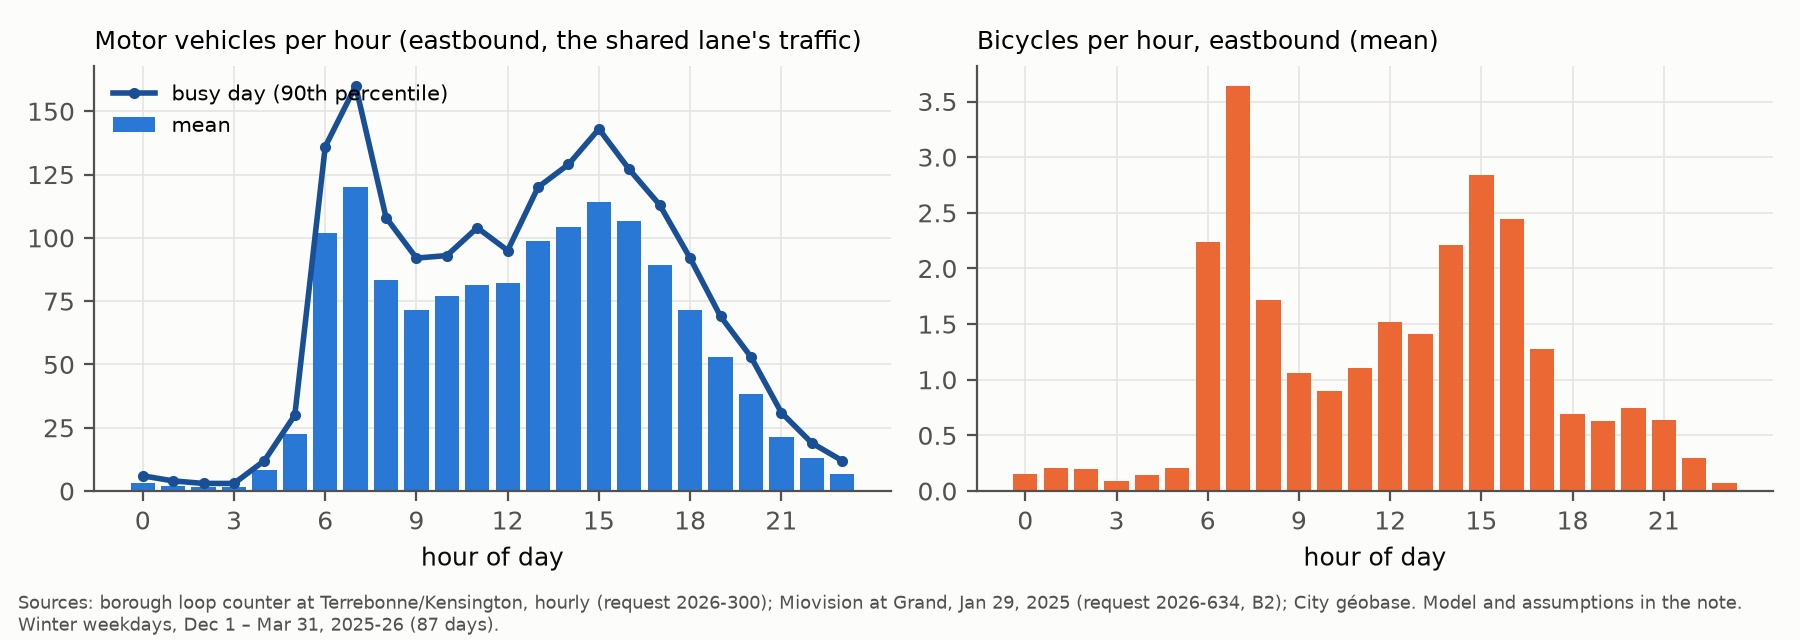
\includegraphics[width=1.0\textwidth]{figures/hourly_flows_en.png}\caption{Winter weekday flows at Kensington, by hour. Morning peak 07:00--08:00: 120 motor vehicles (busy day 160), 3.6 eastbound bicycles; afternoon peak 15:00--16:00: 114 (busy day 143).}\end{figure}
As a check, the Miovision count at Grand gives 128 eastbound cars an hour between 07:00 and 09:00 on January 29, 2025, close to the counter\textquoteright{}s winter mean.

\section{Model}
A cyclist rides at average speed $v_b$; the cars behind would average $v_c > v_b$; both speeds include the stops. Cars pass the counter at $q$ vehicles an hour. Per kilometre the cyclist rides, the cars that catch up number
\[ \lambda = q\left(\frac{1}{v_b} - \frac{1}{v_c}\right). \]
With no passing they queue. A queued car leaves when it turns off at a cross street, with probability $s$ at each one; with $n$ cross streets per kilometre, $\mu = s\,n$, and the expected queue after $x$\,km is
\[ N(x) = \frac{\lambda}{\mu}\left(1 - e^{-\mu x}\right), \]
which tends to $\lambda/\mu$ on a long street and to $\lambda x$ when no one turns off. A Monte Carlo simulation of the same process (catch-ups as a Poisson process along the cyclist\textquoteright{}s path, each queued car turning off with probability $s$ at each of the actual cross streets after Cavendish; 20,000 runs) gives the spread around the expectation.

\begin{table}[htbp]\centering\small
\begin{tabular}{lrrrrrrrr}\toprule
case & $q$ (veh/h) & $v_b$ & $v_c$ & $s$ & caught /km & \multicolumn{3}{c}{expected queue after} \\
 & & (km/h) & (km/h) & & & 0.5\,km & 1\,km & 1.5\,km \\\midrule
low & 100 & 18 & 22 & 12\,\% & 1.0 & 0.4 & 0.6 & 0.7 \\
central & 120 & 15 & 25 & 7\,\% & 3.2 & 1.3 & 2.2 & 2.8 \\
high & 160 & 12 & 28 & 4\,\% & 7.6 & 3.4 & 6.1 & 8.4 \\
\bottomrule\end{tabular}
\caption{The three cases. Central: the mean winter morning peak. High: a busy morning (90th percentile), a slow cyclist on snow, fast cars, few turning off. Low: light traffic, a fast cyclist, slow cars, many turning off.}\end{table}

\section{Results}
\begin{figure}[htbp]\centering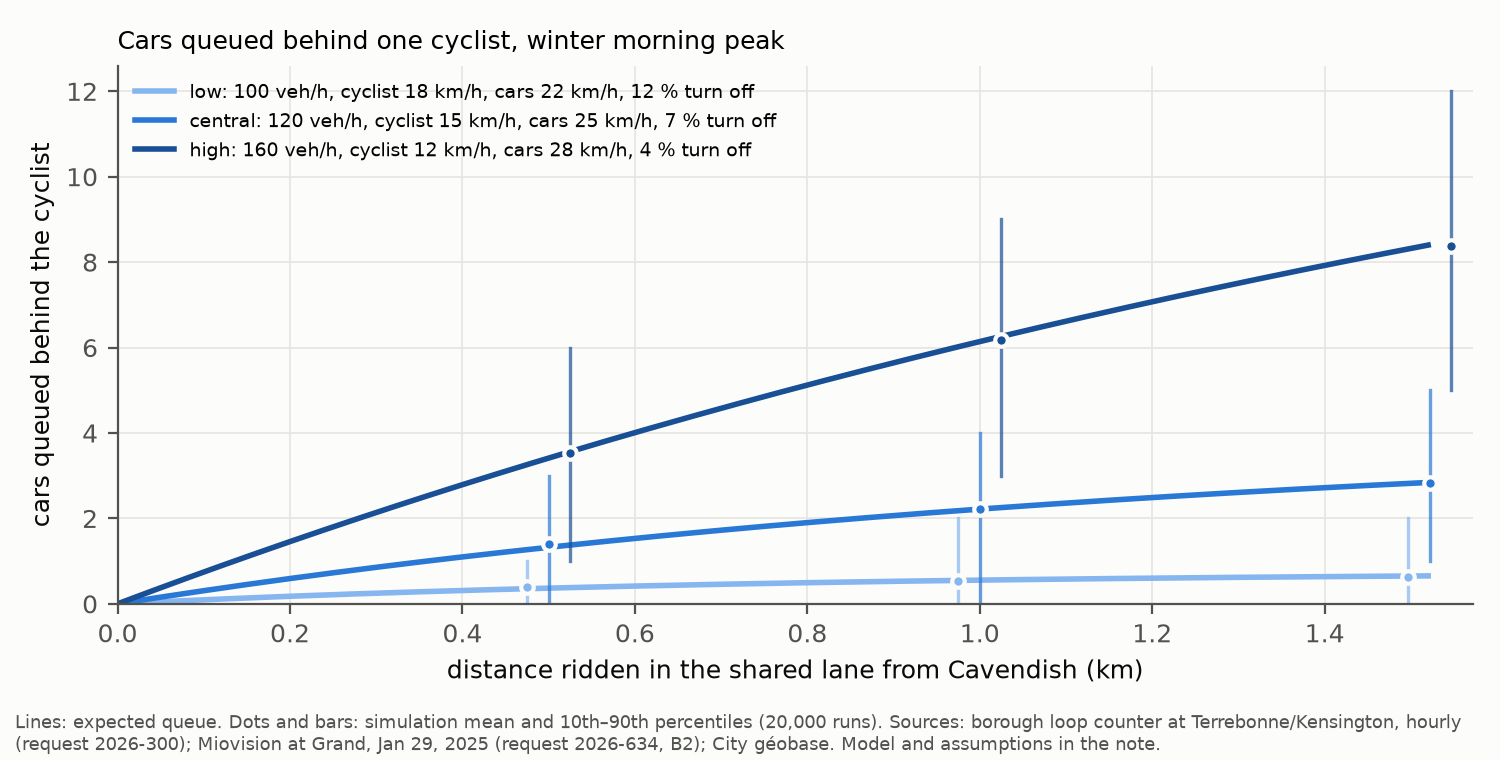
\includegraphics[width=1.0\textwidth]{figures/queue_by_distance_en.png}\caption{Cars queued behind one cyclist riding east from Cavendish, by distance, in the three cases.}\end{figure}
In the central case a cyclist has 2.2 cars behind after 1\,km and 2.8 at Girouard; in the simulation the queue at Girouard has median 3 and 10th--90th percentiles 1--5, and the cyclist reaches Girouard with no car behind in 6\,\% of runs. Averaged over the ride, 1.7 cars follow. On a busy morning with a slow cyclist the queue at Girouard is 8.4 (percentiles 5--12); on a quiet morning with a fast cyclist, under one.

\begin{table}[htbp]\centering\small
\begin{tabular}{lrrrrrr}\toprule
case & km & mean & median & 10th--90th & no car behind & mean over the ride \\\midrule
low & 0.5 & 0.4 & 0 & 0--1 & 67\,\% & 0.2 \\
low & 1 & 0.5 & 0 & 0--2 & 58\,\% & 0.3 \\
low & 1.5 & 0.6 & 0 & 0--2 & 54\,\% & 0.4 \\
central & 0.5 & 1.4 & 1 & 0--3 & 24\,\% & 0.7 \\
central & 1 & 2.2 & 2 & 0--4 & 11\,\% & 1.3 \\
central & 1.5 & 2.8 & 3 & 1--5 & 6\,\% & 1.7 \\
high & 0.5 & 3.5 & 3 & 1--6 & 3\,\% & 1.8 \\
high & 1 & 6.2 & 6 & 3--9 & 0\,\% & 3.3 \\
high & 1.5 & 8.4 & 8 & 5--12 & 0\,\% & 4.7 \\
\bottomrule\end{tabular}
\caption{Simulation, 20,000 runs per case and distance.}\end{table}

\textbf{The drivers\textquoteright{} side.} About 3.6 eastbound cyclists pass Kensington in the morning peak hour. In the central case each is caught by 3.2 cars per kilometre, so about 12 of the 120 cars of that hour (10\,\%) end up behind a cyclist for part of their trip, each losing at most 1.6\,min per kilometre followed. The queue is a constant presence for the cyclist and an occasional one for drivers.

\begin{figure}[htbp]\centering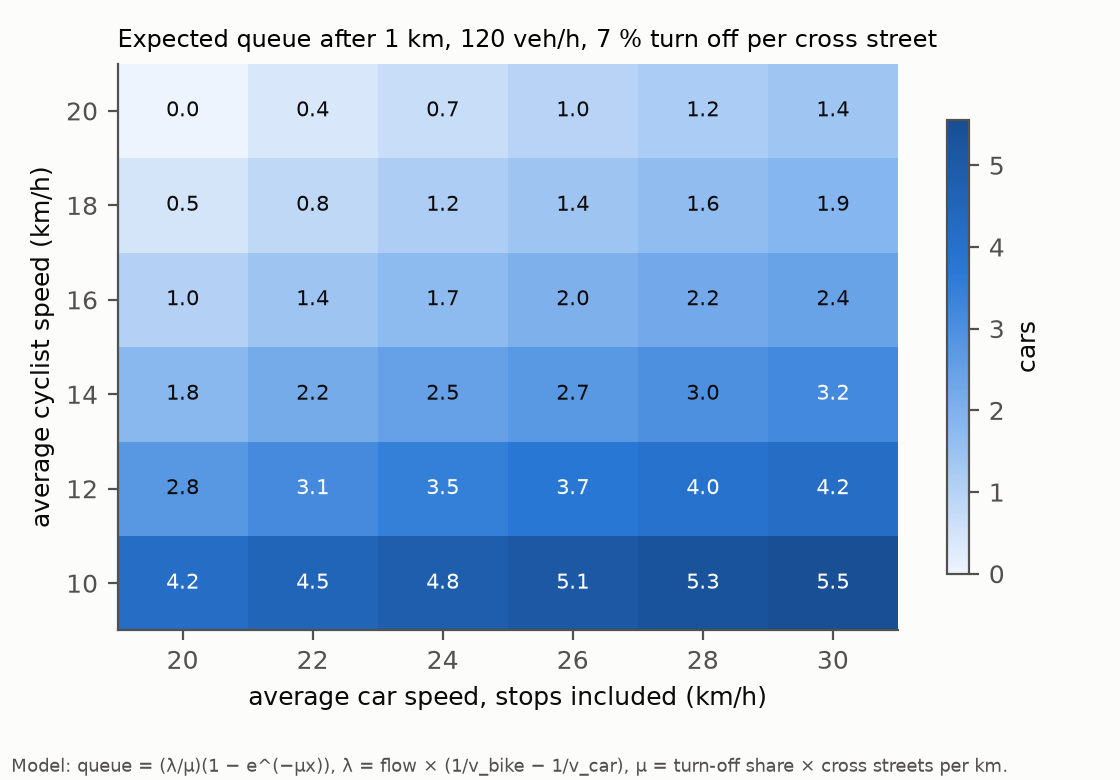
\includegraphics[width=0.72\textwidth]{figures/sensitivity_1km_en.png}\caption{Expected queue after 1\,km at the central flow and turn-off share, by the two speeds.}\end{figure}
The result depends most on the gap between the two speeds: at the central flow, the queue after 1\,km ranges from none, when the cars are no faster than the cyclist, to 5.5 cars with a 10\,km/h cyclist and 30\,km/h cars.

\section{What the estimate leaves out}
\begin{itemize}
\item \textbf{Speeds.} No speed was measured on Terrebonne for either mode. The cases bracket plausible averages with the all-way stops and signals of the street; winter conditions slow cyclists more than cars.
\item \textbf{Turning off.} One intersection (Grand, a boulevard) was measured; the local cross streets, mostly one-way, are assumed to take fewer cars.
\item \textbf{Passing.} The model assumes no pass. Where a driver judges there is room (art.~496.3 on a vélorue), some cars will pass, shortening the queue at the cost of closer passes.
\item \textbf{Several cyclists, snow, the west half.} Cyclists are treated one at a time; snowbanks along parked cars narrow the lane further; west of Cavendish the shared direction is westbound and there is no motor-vehicle count comparable to the Kensington loop, so the estimate covers the east half only.
\item \textbf{Uniform flow.} The counter\textquoteright{}s flow at Kensington is taken to hold along the whole stretch; in fact cars enter and leave at every cross street, so the flow is lower near Cavendish and may differ near Girouard.
\end{itemize}

\section{Reproduction}
\texttt{queue\_analysis.py} reads the two released workbooks from the sibling repository Terrebonne-access-requests (requests 2026-300 and 2026-634) and the street frame of the 1954 plans folder, and writes \texttt{summary.json}, the tables and the figures; \texttt{build\_docs.py} writes this note, the deck and the lay abstracts from \texttt{summary.json}.
\end{document}
